%<<echo=FALSE>>=
%OLD <- options(width=90)
%@
%<<echo=FALSE>>=
%options(OLD) 
%@

\documentclass{beamer}\usepackage[]{graphicx}\usepackage[]{color}
%% maxwidth is the original width if it is less than linewidth
%% otherwise use linewidth (to make sure the graphics do not exceed the margin)
\makeatletter
\def\maxwidth{ %
  \ifdim\Gin@nat@width>\linewidth
    \linewidth
  \else
    \Gin@nat@width
  \fi
}
\makeatother

\definecolor{fgcolor}{rgb}{0.102, 0.102, 0.102}
\newcommand{\hlnum}[1]{\textcolor[rgb]{0.2,0.2,0.2}{#1}}%
\newcommand{\hlstr}[1]{\textcolor[rgb]{0.2,0.2,0.2}{#1}}%
\newcommand{\hlcom}[1]{\textcolor[rgb]{0.302,0.302,0.302}{\textit{#1}}}%
\newcommand{\hlopt}[1]{\textcolor[rgb]{0.102,0.102,0.102}{#1}}%
\newcommand{\hlstd}[1]{\textcolor[rgb]{0.102,0.102,0.102}{#1}}%
\newcommand{\hlkwa}[1]{\textcolor[rgb]{0.102,0.102,0.102}{#1}}%
\newcommand{\hlkwb}[1]{\textcolor[rgb]{0.102,0.102,0.102}{#1}}%
\newcommand{\hlkwc}[1]{\textcolor[rgb]{0.2,0.2,0.2}{#1}}%
\newcommand{\hlkwd}[1]{\textcolor[rgb]{0.102,0.102,0.102}{\textbf{#1}}}%

\usepackage{framed}
\makeatletter
\newenvironment{kframe}{%
 \def\at@end@of@kframe{}%
 \ifinner\ifhmode%
  \def\at@end@of@kframe{\end{minipage}}%
  \begin{minipage}{\columnwidth}%
 \fi\fi%
 \def\FrameCommand##1{\hskip\@totalleftmargin \hskip-\fboxsep
 \colorbox{shadecolor}{##1}\hskip-\fboxsep
     % There is no \\@totalrightmargin, so:
     \hskip-\linewidth \hskip-\@totalleftmargin \hskip\columnwidth}%
 \MakeFramed {\advance\hsize-\width
   \@totalleftmargin\z@ \linewidth\hsize
   \@setminipage}}%
 {\par\unskip\endMakeFramed%
 \at@end@of@kframe}
\makeatother

\definecolor{shadecolor}{rgb}{.97, .97, .97}
\definecolor{messagecolor}{rgb}{0, 0, 0}
\definecolor{warningcolor}{rgb}{1, 0, 1}
\definecolor{errorcolor}{rgb}{1, 0, 0}
\newenvironment{knitrout}{}{} % an empty environment to be redefined in TeX

\usepackage{alltt}% regular slides (with pauses)
%\documentclass[handout]{beamer}% handout (no pauses)

%%%%%%%%%%%%%%%%%%%%%%%%%%%%%%%%%%%%%%%%%%%%%%%%%%%%%%%%%%%%%%%%%%%%%%%%%
%%%%%%% Change the lecture information here %%%%%%%%%%%%%%%%
\def\chapnum{Week \#5}
\title{STAT234: Lecture 8 - Two groups comparison}
\author{Kushal K. Dey}
\date{}
%%%%%%%%%%%%%%%%%%%%%%%%%%%%%%%%%%%%%%%%%%%%%%%%%%%%%%%%%%%%%%%%%%%%%%%%%

%%%%%% Start of suggested definitions and packages %%%%%%%%%%%%
%%%%%% Do not change unless you really know what you are doing %%%%%%%%%%
%%%%%%%%%%%%%%%%%%%%%%%%%%%%%%%%%%%%%%%%%%%%%%%%%%%%%%%%%%%%%%%%%%%%%%%%%

\usepackage{enumerate}
\usepackage{amsmath, bbm}
\usepackage[misc]{ifsym} % for the dice symbol \Cube{}
\usepackage[latin1]{inputenc}
\usepackage{hyperref}
\usepackage{multirow}

%\usepackage{comment}
%\usepackage{pstricks}
%\usepackage{graphicx}
%\usepackage{booktabs}
%\usepackage{pgfpages}
%\pgfpagesuselayout{2 on 1}[a4paper,border shrink=3mm]
%\pgfpagesuselayout{4 on 1}[a4paper,landscape,border shrink=3mm

\usepackage{setspace}
\ifdefined\knitrout
  \renewenvironment{knitrout}{\begin{spacing}{0.75}\begin{tiny}}{\end{tiny}\end{spacing}}
\else
\fi

%%%%%%%%%%%%%%% Defined Shortcuts (macros) %%%%%%%%%%%%%
% parameters and statistics
\newcommand{\xbar}{\overline{x}}
\newcommand{\Xbar}{\overline{X}}
\newcommand{\ybar}{\overline{y}}
\newcommand{\Ybar}{\overline{Y}}
\newcommand{\dbar}{\overline{d}}
\newcommand{\Dbar}{\overline{D}}
\newcommand{\zbar}{\overline{z}}
\newcommand{\Zbar}{\overline{Z}}
\newcommand{\ehat}{\widehat{\epsilon}}
\newcommand{\yhat}{\widehat{y}}
\newcommand{\Yhat}{\widehat{Y}}
\newcommand{\betaa}{{\beta_0}}
\newcommand{\betab}{{\beta_1}}
\newcommand{\betac}{{\beta_2}}
\newcommand{\betad}{{\beta_3}}
\newcommand{\BETA}{{\boldsymbol\beta}}
\newcommand{\betahata}{\widehat{\beta_0}}
\newcommand{\betahatb}{\widehat{\beta_1}}
\newcommand{\betahatc}{\widehat{\beta_2}}
\newcommand{\betahatd}{\widehat{\beta_3}}
\newcommand{\bhat}{\widehat{b}}
\newcommand{\btilde}{\widetilde{b}}
\newcommand{\ahat}{\widehat{a}}
\newcommand{\atilde}{\widetilde{a}}
\newcommand{\rss}{\mathit{SSE}}
\newcommand{\sigmahat}{\widehat{\sigma}}
\newcommand{\betahat}{\widehat{\beta}}
\newcommand{\thetahat}{\widehat{\theta}}
\newcommand{\phat}{\widehat{p}}
\newcommand{\pihat}{\widehat{\pi}}
\newcommand{\muhat}{\widehat{\mu}}
% real numbers and integers
\newcommand{\reals}{\mathbbm{R}}
\newcommand{\integers}{\mathbbm{N}}
%distributions
\newcommand{\normal}{\textsf{Norm}}
\newcommand{\Bin}{\textsf{Binom}}
\newcommand{\Uni}{\textsf{Unif}}
\newcommand{\Poisson}{\textsf{Pois}}
\newcommand{\Exp}{\textsf{Exp}}
\newcommand{\Beta}{\textsf{Beta}}
\newcommand{\iid}{\stackrel{\mathrm{iid}}{\sim}}
% probability and expected value
\newcommand{\rv}{r.v.\ }
\newcommand{\prob}{{\rm P}}
\newcommand{\mean}{\mathrm{E}}
\newcommand{\var}{\mathrm{Var}}
\newcommand{\Var}{\mathrm{Var}}
\newcommand{\cov}{\mathrm{Cov}}
\newcommand{\corr}{\mathop{\mathrm{Corr}}}
% measures of spread
\newcommand{\IQR}{\textit{IQR}}
\newcommand{\SAD}{\textit{SAD}}
\newcommand{\MAD}{\textit{MAD}}
\newcommand{\SSD}{\textit{SSD}}
\newcommand{\MSD}{\textit{MSD}}
\newcommand{\RMSD}{\textit{RMSD}}
\newcommand{\MSE}{\textit{MSE}}
\newcommand{\MSR}{\textit{MSR}}
% formatting code and such
\providecommand{\variable}[1]{}
\renewcommand{\variable}[1]{{\color{green!50!black}\texttt{#1}}}
\providecommand{\function}[1]{}
\renewcommand{\function}[1]{{\color{purple!75!blue}\texttt{\StrSubstitute{#1}{()}{}()}}}
\providecommand{\option}[1]{}
\renewcommand{\option}[1]{{\color{brown!80!black}\texttt{#1}}}
\providecommand{\pkg}[1]{}
\renewcommand{\pkg}[1]{{\color{red!80!black}\texttt{#1}}}
\providecommand{\code}[1]{}
\renewcommand{\code}[1]{{\color{blue!80!black}\texttt{#1}}}

%%%%%%%%%
% Changed by Kushal K Dey, University of Chicago
%\providecommand{\file}[1]{}
%\renewcommand{\file}[1]{{\tt #1}}
\providecommand{\file}[1]{}
\renewcommand{\file}[1]{{\color{orange!80!black}\texttt{#1}}}
%\providecommand{\dataframe}[1]{}
%\renewcommand{\dataframe}[1]{{\color{blue!80!black}\texttt{#1}}}
\providecommand{\dataframe}[1]{}
\renewcommand{\dataframe}[1]{{\color{cyan!80!black}\texttt{#1}}}
%%%%%%%%%

% other
\def\Sum{\sum\nolimits}
\def\b#1{\fboxsep=0pt\colorbox{black}{\color{white}\Cube{#1}}}
\def\w#1{\Cube{#1}}
%%%%%%%%%%%% End of shortcuts (macros) ##############

%%%%%%%%% One way to hide answers until you want to show them %%%%%%%%%
\def\Hide#1#2{\ul{~~~\onslide<#1>{\alert{#2}}~~~}}
\def\hide#1#2{\ul{~~\onslide<#1>{\alert{#2}}~~}}
\def\hid#1#2{\onslide<#1>{\alert{#2}}}
% Choose the color of answers here too
\setbeamercolor{alerted text}{fg=darkgray} 
%\setbeamercolor{alerted text}{fg=black} 

%------Centered Page Number Setup ------
\defbeamertemplate{footline}{centered page number}
{%
  \hspace*{\fill}%
  %\usebeamercolor[fg]{page number in head/foot}%
  %\usebeamerfont{page number in head/foot}%
  \tiny \chapnum: Page \insertframenumber\, of \inserttotalframenumber%
  \hspace*{\fill}\vskip2pt%
}
%\setbeamertemplate{footline}{\hfill\insertframenumber/\inserttotalframenumber}
\setbeamertemplate{footline}[centered page number]
%--------------------------------

%\usetheme{Copenhagen}
\setbeamertemplate{navigation symbols}{}
\usepackage[english]{babel}
\def\ul{\underline}
\linespread{1.1}
% or whatever



%\parskip=0pt
\IfFileExists{upquote.sty}{\usepackage{upquote}}{}
\begin{document}%large

%<<setup, include=FALSE, cache=FALSE>>=
%options(replace.assign=TRUE,width=90, digits=4)
%opts_chunk$set(fig.path='figure/graphics-', cache.path='cache/graphics-', fig.align='center', fig.width=8, fig.height=4.5, fig.show='as.is', out.width='0.9\\linewidth', cache=FALSE, par=TRUE, size = 'tiny', tidy=TRUE, cache.extra=rand_seed)
%knit_hooks$set(par=function(before, options, envir){
%if (before && options$fig.show!='none') par(mar=c(4,4,.1,.1),cex.lab=.95,cex.axis=.9,mgp=c(2,.7,0),tcl=-.3)
%}, document = function(x) {
%  gsub('\\\\(begin|end)\\{kframe\\}', '', x)
%}, crop=hook_pdfcrop)
%@
%<<setup2, include=FALSE, cache=FALSE>>=
%knit_theme$set("print")
%@


%%%%%%%%%%%%%%%%%%%%%%%%%%%%%%%%%%%%%%%%%%%%%%%%%%%%%%%%%%%%%%%%%%%%%%%%%
%%%%%%%%%%%%%%%%%%%%%%%%%%%%%%%%%%%%%%%%%%%%%%%%%%%%%%%%%%%%%%%%%%%%%%%%%
%%%%%% End of suggested definitions and packages %%%%%%%%%%%%

%------------------------------------------------------------------
%------------------------------------------------------------------

%%%%%%%%%% Title frame (optional) %%%%%%%%%%%%%
\begin{frame}{}
\maketitle
\end{frame}
%%%%%%%%%%%%%%%%%%%%%%%%%%%%%%%%%%%%%%%%%%%%%%%

%%%%%%%%%%%%%% Begin slides here %%%%%%%%%%%%%%

%%%%%%%%%%%%%%%%%%%%%%%%%%%%%%%%%%%%%%%%%%%%%%%
\begin{frame}{Today's plan}
%%%%%%%%%%%%%%%%%%%%%%%%%%%%%%%%%%%%%%%%%%%%%%%

\begin{itemize}
\item Comparing two distributions \pause
\item Two sample $t$-test for proportions \pause 
\item Two sample $t$-test for means \pause
\item Matched pair $t$-test vs Pooled $t$- test \pause
\end{itemize}
\end{frame}
%%%%%%%%%%%%%%%%%%%%%%%%%%%%%%%%%%%%%%%%%%%%%%%


%%%%%%%%%%%%%%%%%%%%%%%%%%%%%%%%%%%%%%%%%%%%%%%
\begin{frame}{More importantly !}
%%%%%%%%%%%%%%%%%%%%%%%%%%%%%%%%%%%%%%%%%%%%%%%


\includegraphics[width=\textwidth,keepaspectratio]{final.png} 

\pause 
\begin{center}
\color[rgb]{1,0,0}{\bf Compare Midterm and Finals}
\end{center}

\end{frame}
%%%%%%%%%%%%%%%%%%%%%%%%%%%%%%%%%%%%%%%%%%%%%%%



%%%%%%%%%%%%%%%%%%%%%%%%%%%%%%%%%%%%%%%%%%%%%%%
\begin{frame}
%%%%%%%%%%%%%%%%%%%%%%%%%%%%%%%%%%%%%%%%%%%%%%%

\frametitle{What are the concerns?} 

\begin{itemize}

\item What is the difficulty level of the final paper? 

\item Did good in homeworks and the exams. Do you think I can solve all the problems? 

\item Is it going to be more difficult? 

\end{itemize}

\end{frame}
%%%%%%%%%%%%%%%%%%%%%%%%%%%%%%%%%%%%%%%%%%%%%%%

%%%%%%%%%%%%%%%%%%%%%%%%%%%%%%%%%%%%%%%%%%%%%%%
\begin{frame}
%%%%%%%%%%%%%%%%%%%%%%%%%%%%%%%%%%%%%%%%%%%%%%%

\frametitle{Looking at previous year's data}

\begin{table}[!ht]
\caption{}
\centering
\label{tab:data}
\vspace{0.1in}
\begin{tabular}{c c c}
\hline
Student's name & Midterm Score & Final Score \\
\hline\hline
S & 92  & 52 \\ 
A & 36 &  49 \\ 
C & 32 & 40 \\ 
H & 96 & 75 \\ 
I & 87 & 86 \\ 
N & 72 & 74 \\ 
\hline
\end{tabular}
\end{table}


\end{frame}
%%%%%%%%%%%%%%%%%%%%%%%%%%%%%%%%%%%%%%%%%%%%%%%

%%%%%%%%%%%%%%%%%%%%%%%%%%%%%%%%%%%%%%%%%%%%%%%
\begin{frame}
%%%%%%%%%%%%%%%%%%%%%%%%%%%%%%%%%%%%%%%%%%%%%%%
\frametitle{Formulate the problem}


\begin{itemize}

\item $X$ - pre-final scores, $Y$ - final scores 

\item Need to Compare them 

\item Consider $X_1,X_2,\hdots,X_n \sim N(\mu_1,\sigma_1^2)$ and $Y_1,Y_2,\hdots,Y_n\sim N(\mu_2,\sigma_2^2)$ 

\item We need to test whether $\mu_1$ and $\mu_2$ are same. \pause

\end{itemize}

\begin{center}
What is the null hypothesis? Alternate? What are the assumptions?
\end{center}

\end{frame}
%%%%%%%%%%%%%%%%%%%%%%%%%%%%%%%%%%%%%%%%%%%%%%%

%%%%%%%%%%%%%%%%%%%%%%%%%%%%%%%%%%%%%%%%%%%%%%%
\begin{frame}
%%%%%%%%%%%%%%%%%%%%%%%%%%%%%%%%%%%%%%%%%%%%%%%

\frametitle{Solve the problem}

Test $H_0:\mu_1-\mu_2=0$ against $H_1:\mu_1-\mu_2 > (\ne) 0$ 

\begin{itemize}

\item What are the assumptions?

\item What should the test statistics be?

\item What is the distribution of the test statistics? 

\end{itemize}

\end{frame}
%%%%%%%%%%%%%%%%%%%%%%%%%%%%%%%%%%%%%%%%%%%%%%%

%%%%%%%%%%%%%%%%%%%%%%%%%%%%%%%%%%%%%%%%%%%%%%%
\begin{frame}
%%%%%%%%%%%%%%%%%%%%%%%%%%%%%%%%%%%%%%%%%%%%%%%

\frametitle{Assumptions}

\begin{itemize}
\item $X_1,X_2,\hdots,X_n \sim N(\mu_1,\sigma_1^2)$ 
\item $Y_1,Y_2,\hdots,Y_n\sim N(\mu_2,\sigma_2^2)$ 
\item $X_i,Y_i$ are not independent. Why? \pause Let the correlation be $\rho$ (population parameter, same for all pairs)
\item So, $cov(X_i,Y_i)=\rho\sigma_1\sigma_2$
\end{itemize}

\end{frame}
%%%%%%%%%%%%%%%%%%%%%%%%%%%%%%%%%%%%%%%%%%%%%%%


%%%%%%%%%%%%%%%%%%%%%%%%%%%%%%%%%%%%%%%%%%%%%%%
\begin{frame}
%%%%%%%%%%%%%%%%%%%%%%%%%%%%%%%%%%%%%%%%%%%%%%%

\frametitle{Statistical solution}

Test $H_0:\mu_1-\mu_2=0$ against $H_1:\mu_1-\mu_2 > (\ne) 0$ 

\vspace{0.3cm}

\begin{itemize}


\item $E(\bar X-\bar Y)=\mu_1-\mu_2$ 

\item $var(\bar X-\bar Y)=\frac1n(\sigma_1^2+\sigma_2^2-2\rho\sigma_1\sigma_2)$ 

\item What is the distribution of $\bar X-\bar Y$? 

\item Estimate of the variance?

\end{itemize}

\end{frame}
%%%%%%%%%%%%%%%%%%%%%%%%%%%%%%%%%%%%%%%%%%%%%%%


%%%%%%%%%%%%%%%%%%%%%%%%%%%%%%%%%%%%%%%%%%%%%%%
\begin{frame}
%%%%%%%%%%%%%%%%%%%%%%%%%%%%%%%%%%%%%%%%%%%%%%%

\frametitle{Statistical solution}

\begin{itemize}

\item Define $W_i=X_i-Y_i$ 

\item Then, we get 
\begin{align}
E(W_i) &=& \mu_1-\mu_2=\mu \qquad \text{and} \\
var(W_i) &=& \sigma_1^2+\sigma_2^2-2\rho\sigma_1\sigma_2=\sigma^2 \qquad \text{(say)}
\end{align} 

\item Also note that $\bar W = \bar X - \bar Y$

\end{itemize}

\end{frame}
%%%%%%%%%%%%%%%%%%%%%%%%%%%%%%%%%%%%%%%%%%%%%%%

%%%%%%%%%%%%%%%%%%%%%%%%%%%%%%%%%%%%%%%%%%%%%%%
\begin{frame}
%%%%%%%%%%%%%%%%%%%%%%%%%%%%%%%%%%%%%%%%%%%%%%%

\frametitle{The reformulated problem}

\uncover<1->{$W_1,W_2,\hdots,W_n$ are i.i.d. random variables with mean $\mu$ and unknown variance $\sigma^2$. Test
$$H_0:\mu_{W}=0 \qquad \text{against} \qquad H_1:\mu_{W} > (\ne) 0$$}


\pause
\uncover<2->{\begin{center}
You know it!
\end{center}}

\uncover<3->{\begin{center}
 That is simply a one sample t-test. $H_0:\mu=0$ against proper alternative. It is called Matched pair t-test.
\end{center}}



\end{frame}
%%%%%%%%%%%%%%%%%%%%%%%%%%%%%%%%%%%%%%%%%%%%%%%

%%%%%%%%%%%%%%%%%%%%%%%%%%%%%%%%%%%%%%%%%%%%%%%
\begin{frame}
%%%%%%%%%%%%%%%%%%%%%%%%%%%%%%%%%%%%%%%%%%%%%%%

Since $W_{i}=X_{i} - Y_{i}$, and $X_{i}$ and $Y_{i}$ are normal random variables,
hence $W_i$ also normal. \pause

$$ W_i \sim N (\mu_{W}, \sigma^2_{W}) $$ \pause

$$ \mu_{W} = \mu_1 - \mu_2 $$ \pause

$$ \sigma^2_{W} = \sigma_1^2+\sigma_2^2-2\rho\sigma_1\sigma_2=\sigma^2 $$ \pause

Under $H_{0}$, we get 

$$ W_{1}, W_{2}, \cdots, W_{n} \sim N(0, \sigma^2_{W}) $$

\end{frame}
%%%%%%%%%%%%%%%%%%%%%%%%%%%%%%%%%%%%%%%%%%%%%%%

%%%%%%%%%%%%%%%%%%%%%%%%%%%%%%%%%%%%%%%%%%%%%%%
\begin{frame}
%%%%%%%%%%%%%%%%%%%%%%%%%%%%%%%%%%%%%%%%%%%%%%%

Under $H_{0}$,

$$ \bar{W} \sim N \left( 0, \frac{\sigma^2_{W}}{n} \right) $$

$$ \frac{\sqrt{n} \bar{W}}{\sigma_{W}} \sim N(0,1) $$

We do not know $\sigma_{W}$, so we replace it by $s_{W}$, 

$$ s^2_{W} : = \frac{1}{n-1} \sum_{i=1}^{n} \left (W_i - \bar{W} \right )^2 $$

What is the distribution of 

$$ \frac{\sqrt{n} \bar{W}}{s_{W}}  $$

\end{frame}
%%%%%%%%%%%%%%%%%%%%%%%%%%%%%%%%%%%%%%%%%%%%%%%

%%%%%%%%%%%%%%%%%%%%%%%%%%%%%%%%%%%%%%%%%%%%%%%
\begin{frame}[fragile]
%%%%%%%%%%%%%%%%%%%%%%%%%%%%%%%%%%%%%%%%%%%%%%%

$$ \frac{\sqrt{n} \bar{W}}{s_{W}}  \sim t_{n-1}  $$

Compute the observed value $\bar{w}$ pf $\bar{W}$ and $s_{w}$- realization of $s_{W}$.

From the data we presented,

\begin{knitrout}\small
\definecolor{shadecolor}{rgb}{1, 1, 1}\color{fgcolor}\begin{kframe}
\begin{alltt}
\hlkwd{set.seed}\hlstd{(}\hlnum{100}\hlstd{)}
\hlstd{x} \hlkwb{<-} \hlkwd{c}\hlstd{(}\hlnum{92}\hlstd{,} \hlnum{36}\hlstd{,} \hlnum{32}\hlstd{,} \hlnum{96}\hlstd{,} \hlnum{87}\hlstd{,} \hlnum{72}\hlstd{)}
\hlstd{y} \hlkwb{<-} \hlkwd{c}\hlstd{(}\hlnum{32}\hlstd{,} \hlnum{49}\hlstd{,} \hlnum{40}\hlstd{,} \hlnum{75}\hlstd{,} \hlnum{86}\hlstd{,} \hlnum{74}\hlstd{)}
\hlstd{W} \hlkwb{<-} \hlstd{x}\hlopt{-}\hlstd{y}
\hlstd{Wbar} \hlkwb{<-} \hlkwd{mean}\hlstd{(W); sW} \hlkwb{<-} \hlkwd{sd}\hlstd{(W)}
\hlstd{tstat} \hlkwb{=} \hlkwd{sqrt}\hlstd{(}\hlkwd{length}\hlstd{(W))}\hlopt{*}\hlstd{Wbar}\hlopt{/}\hlstd{sW}
\end{alltt}
\end{kframe}
\end{knitrout}


\end{frame}
%%%%%%%%%%%%%%%%%%%%%%%%%%%%%%%%%%%%%%%%%%%%%%%

%%%%%%%%%%%%%%%%%%%%%%%%%%%%%%%%%%%%%%%%%%%%%%%
\begin{frame}[fragile]
%%%%%%%%%%%%%%%%%%%%%%%%%%%%%%%%%%%%%%%%%%%%%%%
\frametitle{Resampling distribution}

\begin{knitrout}\small
\definecolor{shadecolor}{rgb}{1, 1, 1}\color{fgcolor}\begin{kframe}
\begin{alltt}
\hlstd{W_new} \hlkwb{<-} \hlstd{W} \hlopt{-} \hlstd{Wbar} \hlopt{+} \hlnum{0}\hlstd{;}
\hlstd{bootstapW} \hlkwb{<-} \hlkwd{replicate}\hlstd{(}\hlnum{10000}\hlstd{,} \hlkwd{sample}\hlstd{(W_new,} \hlkwc{replace}\hlstd{=}\hlnum{TRUE}\hlstd{))}
\hlstd{tstat_boot} \hlkwb{<-} \hlkwd{sqrt}\hlstd{(}\hlkwd{length}\hlstd{(W))}\hlopt{*}
              \hlstd{(}\hlkwd{apply}\hlstd{(bootstapW,} \hlnum{2}\hlstd{, mean)}\hlopt{/}\hlkwd{apply}\hlstd{(bootstapW,}\hlnum{2}\hlstd{, sd))}
\hlkwd{hist}\hlstd{(tstat_boot,} \hlkwc{freq}\hlstd{=}\hlnum{FALSE}\hlstd{)}
\end{alltt}
\end{kframe}

{\centering 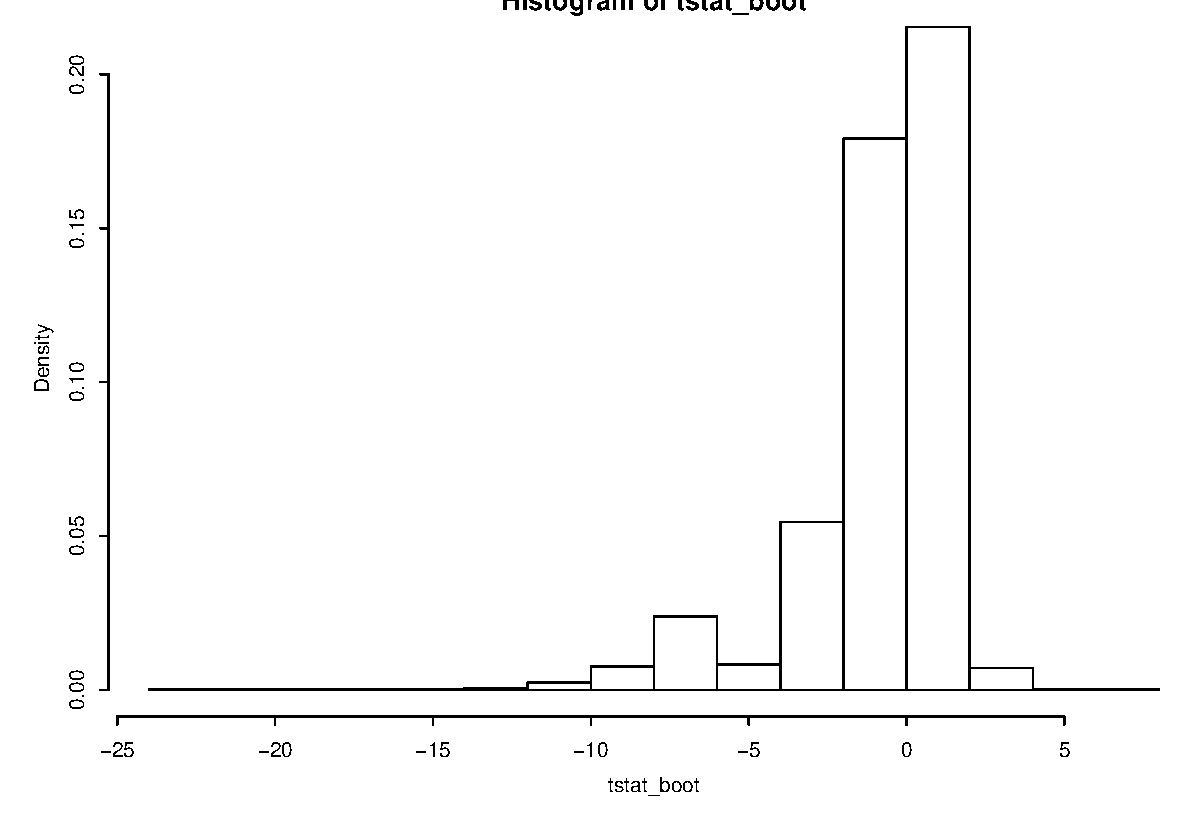
\includegraphics[width=0.99\linewidth]{figure/graphics-unnamed-chunk-2-1} 

}



\end{knitrout}

\end{frame}
%%%%%%%%%%%%%%%%%%%%%%%%%%%%%%%%%%%%%%%%%%%%%%%


%%%%%%%%%%%%%%%%%%%%%%%%%%%%%%%%%%%%%%%%%%%%%%%
\begin{frame}[fragile]
%%%%%%%%%%%%%%%%%%%%%%%%%%%%%%%%%%%%%%%%%%%%%%%
\frametitle{Resampling distribution}

\begin{knitrout}\small
\definecolor{shadecolor}{rgb}{1, 1, 1}\color{fgcolor}\begin{kframe}
\begin{alltt}
\hlkwd{library}\hlstd{(gap)}
\hlkwd{qqfun}\hlstd{(tstat_boot,} \hlstr{"t"}\hlstd{,} \hlkwc{df}\hlstd{=}\hlkwd{length}\hlstd{(W)}\hlopt{-}\hlnum{1}\hlstd{)}
\end{alltt}
\end{kframe}

{\centering 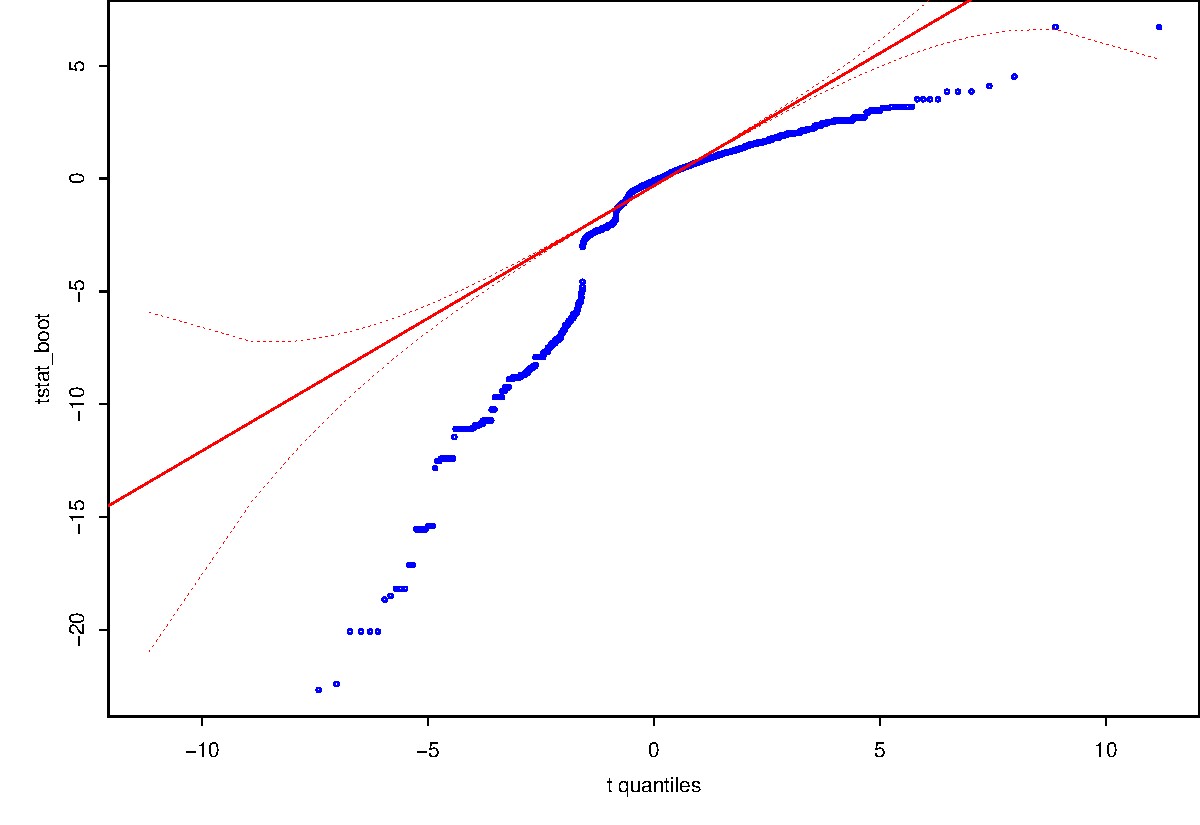
\includegraphics[width=0.99\linewidth]{figure/graphics-unnamed-chunk-3-1} 

}



\end{knitrout}

\end{frame}
%%%%%%%%%%%%%%%%%%%%%%%%%%%%%%%%%%%%%%%%%%%%%%%

%%%%%%%%%%%%%%%%%%%%%%%%%%%%%%%%%%%%%%%%%%%%%%%
\begin{frame}[fragile]
%%%%%%%%%%%%%%%%%%%%%%%%%%%%%%%%%%%%%%%%%%%%%%%
\frametitle{p-value}

\begin{knitrout}\small
\definecolor{shadecolor}{rgb}{1, 1, 1}\color{fgcolor}\begin{kframe}
\begin{alltt}
\hlstd{tstat} \hlkwb{=} \hlkwd{sqrt}\hlstd{(}\hlkwd{length}\hlstd{(W))}\hlopt{*}\hlstd{Wbar}\hlopt{/}\hlstd{sW}
\hlstd{pval_t} \hlkwb{=} \hlnum{1} \hlopt{-} \hlkwd{pt}\hlstd{(tstat,}\hlkwc{df}\hlstd{=}\hlkwd{length}\hlstd{(W)}\hlopt{-}\hlnum{1}\hlstd{)}

\hlstd{pval_boot} \hlkwb{<-} \hlkwd{length}\hlstd{(}\hlkwd{which}\hlstd{(tstat_boot} \hlopt{>} \hlstd{tstat))}\hlopt{/}\hlkwd{length}\hlstd{(tstat_boot)}

\hlstd{pval_t}
\end{alltt}
\begin{verbatim}
[1] 0.2082
\end{verbatim}
\begin{alltt}
\hlstd{pval_boot}
\end{alltt}
\begin{verbatim}
[1] 0.1397
\end{verbatim}
\end{kframe}
\end{knitrout}

\end{frame}
%%%%%%%%%%%%%%%%%%%%%%%%%%%%%%%%%%%%%%%%%%%%%%%

% %%%%%%%%%%%%%%%%%%%%%%%%%%%%%%%%%%%%%%%%%%%%%%%
% \begin{frame}[fragile]
% %%%%%%%%%%%%%%%%%%%%%%%%%%%%%%%%%%%%%%%%%%%%%%%
% 
% \frametitle{R output (one-sided test)}
% 
% \begin{verbatim}
% > data = read.table("data.csv",header=FALSE,sep=",")
% > 
% > W = data[,1] - data[,2]
% > Wbar = mean(W)
% > sW = sd(W)
% > tstat = sqrt(length(W))*Wbar/sW
% > pval = 1 - pt(tstat,df=length(W)-1)
% > 
% > cbind(Wbar,sW,tstat,pval)
%          Wbar      sW    tstat         pval
% [1,] 9.382812 11.2718 6.659317 3.907086e-09
% \end{verbatim}
% 
% \begin{center}
% \color[rgb]{1,0,0} Conclusion : "Yes, we need to study more"
% \end{center}
% 
% \end{frame}
% %%%%%%%%%%%%%%%%%%%%%%%%%%%%%%%%%%%%%%%%%%%%%%%

%%%%%%%%%%%%%%%%%%%%%%%%%%%%%%%%%%%%%%%%%%%%%%%
\begin{frame}[fragile]
%%%%%%%%%%%%%%%%%%%%%%%%%%%%%%%%%%%%%%%%%%%%%%%

\frametitle{A more complicated scenario}

Suppose you sampled 30 students' scores for the midterm exam and 
for the 2012 exam, another person sampled 26 students' scores for the end term.
\pause \newline

You do not know if the 26 students are a different set from 30 students or not.
How do you go about analyzing the data then? \pause \newline

Then we assume if $X_i$ denote midterm score and $Y_i$ the final score, 

\begin{itemize}
\item $X_1,X_2,\hdots,X_{30} \sim N(\mu_1,\sigma_1^2)$ 
\item $Y_1,Y_2,\hdots,Y_{26} \sim N(\mu_2,\sigma_2^2)$ 
\end{itemize}

W assume that $X_i$'s and $Y_i$'s are independent. So, $\rho=cor(X,Y)=0$.


\end{frame}
%%%%%%%%%%%%%%%%%%%%%%%%%%%%%%%%%%%%%%%%%%%%%%%

%%%%%%%%%%%%%%%%%%%%%%%%%%%%%%%%%%%%%%%%%%%%%%%
\begin{frame}[fragile]
%%%%%%%%%%%%%%%%%%%%%%%%%%%%%%%%%%%%%%%%%%%%%%%

\frametitle{Statistical solution}

Test $H_0:\mu_1-\mu_2=0$ against $H_1:\mu_1-\mu_2 > (\ne) 0$  \pause

\vspace{0.3cm}

\begin{itemize}

\item So, our test statistics should be $\bar X-\bar Y$ \pause

\item $E(\bar X-\bar Y)=\mu_1-\mu_2$  \pause

\item $var(\bar X-\bar Y)=(\sigma_1^2/30+\sigma_2^2/26)$  \pause

\item Since we assume independence, the distribution of $\bar X-\bar Y$ is $N(\mu_1-\mu_2,\sigma_1^2/30+\sigma_2^2/26)$ \pause

\item Estimate of the variance: $(s_1^2/30+s_2^2/26)$ \pause

\item What is the distribution of the above estimate?

\end{itemize}

\end{frame}
%%%%%%%%%%%%%%%%%%%%%%%%%%%%%%%%%%%%%%%%%%%%%

%%%%%%%%%%%%%%%%%%%%%%%%%%%%%%%%%%%%%%%%%%%%%
\begin{frame}[fragile]
%%%%%%%%%%%%%%%%%%%%%%%%%%%%%%%%%%%%%%%%%%%%%

\frametitle{More complicated scenario}

Consider the following set-up.

\begin{itemize}
\item $X_1,X_2,\hdots,X_{30} \sim N(\mu_1,\sigma_1^2)$ 
\item $Y_1,Y_2,\hdots,Y_{26} \sim N(\mu_2,\sigma_2^2)$  \pause
\item But we assume that $X_i$'s and $Y_i$'s are independent. Why?\pause So, $\rho=0$.
\end{itemize} 

How to deal with this? - We will consider two different scenarios. \pause
\begin{itemize}
\item two variances are equal
\item variances are not equal
\end{itemize}

\end{frame}
%%%%%%%%%%%%%%%%%%%%%%%%%%%%%%%%%%%%%%%%%%%%%

%%%%%%%%%%%%%%%%%%%%%%%%%%%%%%%%%%%%%%%%%%%%%
\begin{frame}
%%%%%%%%%%%%%%%%%%%%%%%%%%%%%%%%%%%%%%%%%%%%%

\frametitle{Set-up}

We have $X_1,X_2,\hdots,X_n \sim N(\mu_1,\sigma_1^2)$  and $Y_1,Y_2,\hdots,Y_m \sim N(\mu_2,\sigma_2^2)$ \pause

\begin{itemize}
\item Test $H_0: \mu_1-\mu_2=0$ against $H_0: \mu_1-\mu_2\ne 0$ \pause
\item $\sigma_1,\sigma_2$ are unknown \pause
\item You know that an estimate of $\mu_1-\mu_2$ is $\bar X-\bar Y$. So, we should try to find out the distribution of this. \pause
\item The distribution is $$\bar X-\bar Y \sim N(\mu_1-\mu_2,\sigma_1^2/n+\sigma_2^2/m)$$ 
 i.e. $$ \frac{(\bar X-\bar Y)-(\mu_1-\mu_2)}{\sqrt{\sigma_1^2/n+\sigma_2^2/m}} \sim N(0,1)$$
\end{itemize}

\end{frame}
%%%%%%%%%%%%%%%%%%%%%%%%%%%%%%%%%%%%%%%%%%%%%

%%%%%%%%%%%%%%%%%%%%%%%%%%%%%%%%%%%%%%%%%%%%%
\begin{frame}
%%%%%%%%%%%%%%%%%%%%%%%%%%%%%%%%%%%%%%%%%%%%%

\frametitle{Two sample test with equal variance}

Suppose, we have reasons to believe that the variances are equal i.e. $\sigma_1=\sigma_2=\sigma$. Then, we have
$$Z=\frac{(\bar X-\bar Y)-(\mu_1-\mu_2)}{\sigma\sqrt{1/n+1/m}} \sim N(0,1)$$ \pause
\begin{itemize}
\item Clearly, we have to estimate $\sigma^2$. \pause
\item Recall that both $s_X^2$ and $s_Y^2$ are unbiased estimates of $\sigma^2$. We should combine them.
\pause
\end{itemize}


$$ \hat{\sigma^2}: = \frac{(n-1)s_X^2 + (m-1)s_Y^2}{m+n-2} $$

\end{frame}
%%%%%%%%%%%%%%%%%%%%%%%%%%%%%%%%%%%%%%%%%%%%%

%%%%%%%%%%%%%%%%%%%%%%%%%%%%%%%%%%%%%%%%%%%%%
\begin{frame}
%%%%%%%%%%%%%%%%%%%%%%%%%%%%%%%%%%%%%%%%%%%%%

\frametitle{Two sample test with equal variance (contd)}

Test $H_0:\mu_1-\mu_2=0$ against $H_0: \mu_1-\mu_2\ne 0$ and we have

$$Z=\frac{(\bar X-\bar Y)-(\mu_1-\mu_2)}{\sigma\sqrt{1/n+1/m}} \sim N(0,1) $$

$$T=\frac{(\bar X-\bar Y)-(\mu_1-\mu_2)}{\hat{\sigma} \sqrt{1/n+1/m}} \sim t_{n+m-2}$$ \pause


\end{frame}
%%%%%%%%%%%%%%%%%%%%%%%%%%%%%%%%%%%%%%%%%%%%%

%%%%%%%%%%%%%%%%%%%%%%%%%%%%%%%%%%%%%%%%%%%%%
\begin{frame}[fragile]
%%%%%%%%%%%%%%%%%%%%%%%%%%%%%%%%%%%%%%%%%%%%%

\begin{knitrout}\small
\definecolor{shadecolor}{rgb}{1, 1, 1}\color{fgcolor}\begin{kframe}
\begin{alltt}
\hlstd{x} \hlkwb{<-} \hlkwd{rnorm}\hlstd{(}\hlnum{30}\hlstd{,} \hlnum{67}\hlstd{,} \hlnum{10}\hlstd{);}
\hlstd{y} \hlkwb{<-} \hlkwd{rnorm}\hlstd{(}\hlnum{26}\hlstd{,} \hlnum{56}\hlstd{,} \hlnum{10}\hlstd{);}

\hlstd{meanW} \hlkwb{<-} \hlkwd{mean}\hlstd{(x)} \hlopt{-} \hlkwd{mean}\hlstd{(y)}
\hlstd{sX2} \hlkwb{<-} \hlkwd{var}\hlstd{(x); sY2} \hlkwb{<-} \hlkwd{var}\hlstd{(y);}
\hlstd{s2_pool} \hlkwb{<-} \hlstd{((}\hlkwd{length}\hlstd{(x)}\hlopt{-}\hlnum{1}\hlstd{)}\hlopt{*}\hlstd{sX2}
            \hlopt{+} \hlstd{(}\hlkwd{length}\hlstd{(y)}\hlopt{-}\hlnum{1}\hlstd{)}\hlopt{*}\hlstd{sY2)}\hlopt{/}\hlstd{(}\hlkwd{length}\hlstd{(x)}\hlopt{+}\hlkwd{length}\hlstd{(y)}\hlopt{-}\hlnum{2}\hlstd{);}

\hlstd{tstat} \hlkwb{<-} \hlstd{meanW}\hlopt{/} \hlstd{(}\hlkwd{sqrt}\hlstd{(s2_pool)}\hlopt{*}\hlstd{(}\hlkwd{sqrt}\hlstd{(}\hlnum{1}\hlopt{/}\hlstd{(}\hlkwd{length}\hlstd{(x))} \hlopt{+} \hlnum{1}\hlopt{/}\hlstd{(}\hlkwd{length}\hlstd{(y)))));}
\end{alltt}
\end{kframe}
\end{knitrout}

\end{frame}
%%%%%%%%%%%%%%%%%%%%%%%%%%%%%%%%%%%%%%%%%%%%%

%%%%%%%%%%%%%%%%%%%%%%%%%%%%%%%%%%%%%%%%%%%%%
\begin{frame}[fragile]
%%%%%%%%%%%%%%%%%%%%%%%%%%%%%%%%%%%%%%%%%%%%%

\begin{knitrout}\small
\definecolor{shadecolor}{rgb}{1, 1, 1}\color{fgcolor}\begin{kframe}
\begin{alltt}
\hlstd{xboot} \hlkwb{<-} \hlkwd{replicate}\hlstd{(}\hlnum{10000}\hlstd{,} \hlkwd{sample}\hlstd{(}\hlkwd{c}\hlstd{(x,y),} \hlkwd{length}\hlstd{(x),} \hlkwc{replace} \hlstd{=} \hlnum{FALSE}\hlstd{));}
\hlstd{yboot} \hlkwb{<-} \hlkwd{replicate}\hlstd{(}\hlnum{10000}\hlstd{,} \hlkwd{sample}\hlstd{(}\hlkwd{c}\hlstd{(x,y),} \hlkwd{length}\hlstd{(y),} \hlkwc{replace} \hlstd{=} \hlnum{FALSE}\hlstd{));}

\hlstd{mean_wboot} \hlkwb{<-} \hlkwd{colMeans}\hlstd{(xboot)}  \hlopt{-} \hlkwd{colMeans}\hlstd{(yboot)}
\hlstd{sx_boot2} \hlkwb{<-} \hlkwd{apply}\hlstd{(xboot,} \hlnum{2}\hlstd{, var)}
\hlstd{sy_boot2} \hlkwb{<-} \hlkwd{apply}\hlstd{(yboot,} \hlnum{2}\hlstd{, var)}
\hlstd{s_boot2} \hlkwb{<-} \hlstd{((}\hlkwd{length}\hlstd{(x)}\hlopt{-}\hlnum{1}\hlstd{)}\hlopt{*}\hlstd{sx_boot2} \hlopt{+} \hlstd{(}\hlkwd{length}\hlstd{(y)}\hlopt{-}\hlnum{1}\hlstd{)}\hlopt{*}\hlstd{sy_boot2)}\hlopt{/}\hlstd{(}\hlkwd{length}\hlstd{(x)}\hlopt{+}\hlkwd{length}\hlstd{(y)}\hlopt{-}\hlnum{2}\hlstd{);}

\hlstd{tstat_boot} \hlkwb{<-} \hlstd{mean_wboot}\hlopt{/}\hlstd{(}\hlkwd{sqrt}\hlstd{(s_boot2)}\hlopt{*}\hlstd{(}\hlkwd{sqrt}\hlstd{(}\hlnum{1}\hlopt{/}\hlstd{(}\hlkwd{length}\hlstd{(x))} \hlopt{+} \hlnum{1}\hlopt{/}\hlstd{(}\hlkwd{length}\hlstd{(y)))))}
\end{alltt}
\end{kframe}
\end{knitrout}

\end{frame}
%%%%%%%%%%%%%%%%%%%%%%%%%%%%%%%%%%%%%%%%%%%%%

%%%%%%%%%%%%%%%%%%%%%%%%%%%%%%%%%%%%%%%%%%%%%
\begin{frame}[fragile]
%%%%%%%%%%%%%%%%%%%%%%%%%%%%%%%%%%%%%%%%%%%%%

\begin{knitrout}\small
\definecolor{shadecolor}{rgb}{1, 1, 1}\color{fgcolor}

{\centering 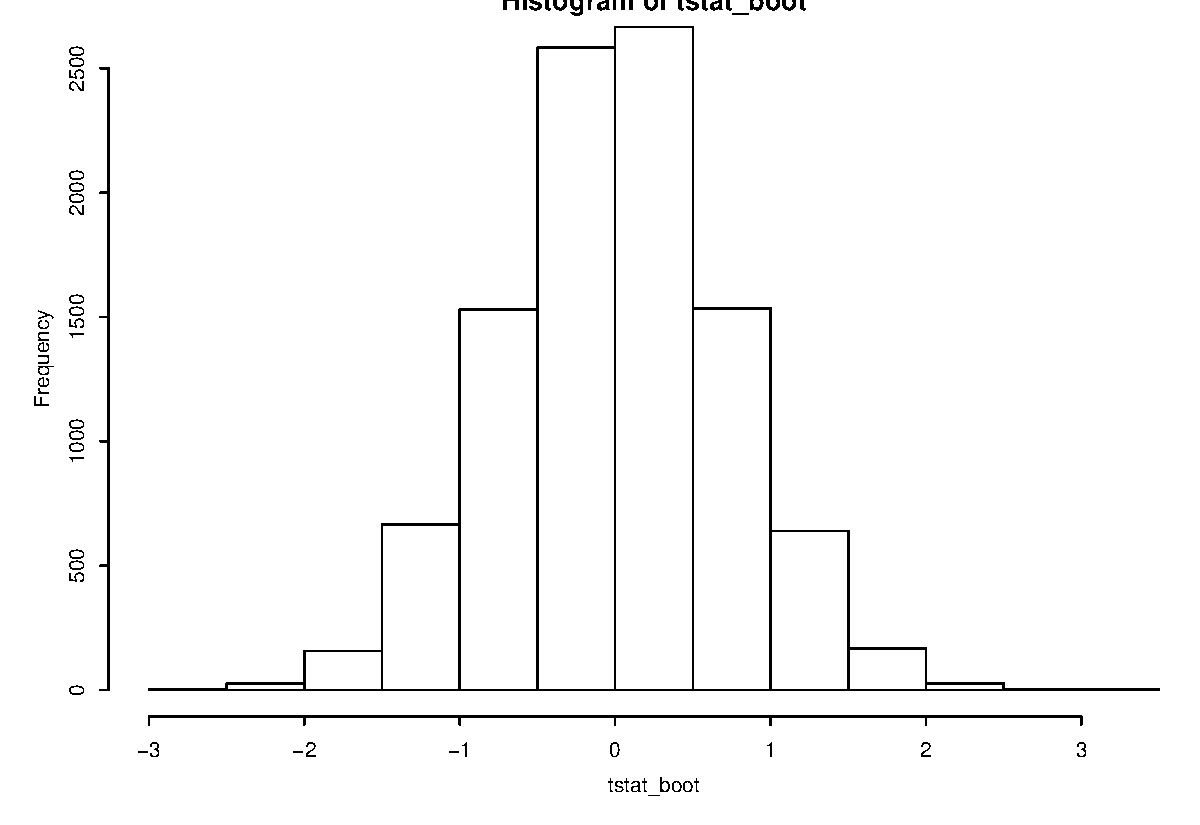
\includegraphics[width=0.99\linewidth]{figure/graphics-unnamed-chunk-7-1} 

}



\end{knitrout}

\end{frame}
%%%%%%%%%%%%%%%%%%%%%%%%%%%%%%%%%%%%%%%%%%%%%

%%%%%%%%%%%%%%%%%%%%%%%%%%%%%%%%%%%%%%%%%%%%%
\begin{frame}[fragile]
%%%%%%%%%%%%%%%%%%%%%%%%%%%%%%%%%%%%%%%%%%%%%
\frametitle{qqplot with t(54)}

\begin{knitrout}\small
\definecolor{shadecolor}{rgb}{1, 1, 1}\color{fgcolor}\begin{kframe}
\begin{alltt}
\hlkwd{library}\hlstd{(gap)}
\hlkwd{qqfun}\hlstd{(tstat_boot,} \hlstr{"t"}\hlstd{,} \hlkwc{df}\hlstd{=}\hlkwd{length}\hlstd{(x)}\hlopt{+}\hlkwd{length}\hlstd{(y)}\hlopt{-}\hlnum{2}\hlstd{)}
\end{alltt}
\end{kframe}

{\centering 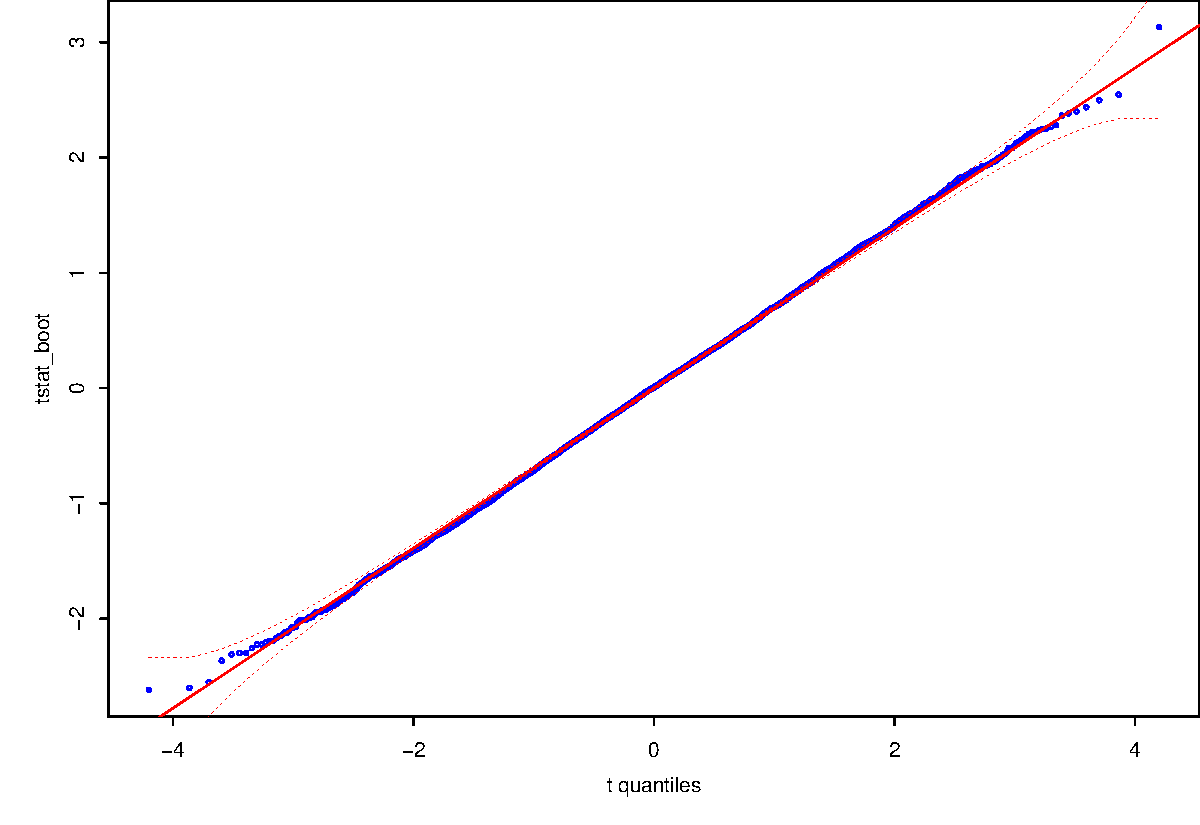
\includegraphics[width=0.99\linewidth]{figure/graphics-unnamed-chunk-8-1} 

}



\end{knitrout}

\end{frame}
%%%%%%%%%%%%%%%%%%%%%%%%%%%%%%%%%%%%%%%%%%%%%

%%%%%%%%%%%%%%%%%%%%%%%%%%%%%%%%%%%%%%%%%%%%%%%
\begin{frame}[fragile]
%%%%%%%%%%%%%%%%%%%%%%%%%%%%%%%%%%%%%%%%%%%%%%%
\frametitle{p-value}

\begin{knitrout}\small
\definecolor{shadecolor}{rgb}{1, 1, 1}\color{fgcolor}\begin{kframe}
\begin{alltt}
\hlstd{tstat} \hlkwb{<-} \hlstd{meanW}\hlopt{/} \hlstd{(}\hlkwd{sqrt}\hlstd{(s2_pool)}\hlopt{*}\hlstd{(}\hlkwd{sqrt}\hlstd{(}\hlnum{1}\hlopt{/}\hlstd{(}\hlkwd{length}\hlstd{(x))} \hlopt{+} \hlnum{1}\hlopt{/}\hlstd{(}\hlkwd{length}\hlstd{(y)))));}
\hlstd{pval_t} \hlkwb{=} \hlnum{1} \hlopt{-} \hlkwd{pt}\hlstd{(tstat,}\hlkwc{df}\hlstd{=}\hlkwd{length}\hlstd{(x)}\hlopt{+}\hlkwd{length}\hlstd{(y)}\hlopt{-}\hlnum{1}\hlstd{)}

\hlstd{pval_boot} \hlkwb{<-} \hlkwd{length}\hlstd{(}\hlkwd{which}\hlstd{(tstat_boot} \hlopt{>} \hlstd{tstat))}\hlopt{/}\hlkwd{length}\hlstd{(tstat_boot)}

\hlstd{pval_t}
\end{alltt}
\begin{verbatim}
[1] 0.0002026
\end{verbatim}
\begin{alltt}
\hlstd{pval_boot}
\end{alltt}
\begin{verbatim}
[1] 0
\end{verbatim}
\end{kframe}
\end{knitrout}

\end{frame}
%%%%%%%%%%%%%%%%%%%%%%%%%%%%%%%%%%%%%%%%%%%%%%%


%%%%%%%%%%%%%%%%%%%%%%%%%%%%%%%%%%%%%%%%%%%%%
\begin{frame}
%%%%%%%%%%%%%%%%%%%%%%%%%%%%%%%%%%%%%%%%%%%%%

\frametitle{Two sample test with equal variance (contd)}

Test $H_0:\mu_1-\mu_2=0$ against $H_0: \mu_1-\mu_2\ne 0$ and our test statistic is
\begin{eqnarray*}
T &=& \frac{(\bar X-\bar Y)-(\mu_1-\mu_2)}{\sigma\sqrt{1/n+1/m}} . \sqrt{\frac{\sigma^2(n+m-2)}{(n-1)s_X^2+(m-1)s_Y^2}} \\
&=& \frac{(\bar X-\bar Y)-(\mu_1-\mu_2)}{S_{XY}\sqrt{1/n+1/m}} \text{ where } S_{XY}^2=\frac{(n-1)s_X^2+(m-1)s_Y^2}{n+m-2}
\end{eqnarray*} \pause
\begin{itemize}
\item $S_{XY}^2=$ Pooled variance
\item For this problem, p-value will be $2P(T\ge |t|)$ where $t$ is the observed value of the statistic and $T\sim t_{n+m-2}$
\end{itemize}

\end{frame}
%%%%%%%%%%%%%%%%%%%%%%%%%%%%%%%%%%%%%%%%%%%%%


%%%%%%%%%%%%%%%%%%%%%%%%%%%%%%%%%%%%%%%%%%%%%
\begin{frame}
%%%%%%%%%%%%%%%%%%%%%%%%%%%%%%%%%%%%%%%%%%%%%

\frametitle{2- sample test (unequal variance) - Behren-Fisher problem}

Suppose, we have reasons to believe that the variances are not equal i.e. $\sigma_1\ne\sigma_2$. Then, we have
$$\bar X-\bar Y \sim N(\mu_1-\mu_2,\sigma_1^2/n+\sigma_2^2/m)$$
\begin{itemize}
\item So, the two population variances must be estimated separately. 
\item Recall that $s_X^2$ and $s_Y^2$ are unbiased estimates of $\sigma_1^2,\sigma_2^2$. We should combine them.
\item The estimate is $$S_{\bar X-\bar Y}^2 = \frac{s_X^2}{n} + \frac{s_Y^2}{m}$$
\item The t statistic to test our hypothesis is:
$$T = \frac{(\bar X-\bar Y)-(\mu_1-\mu_2)}{S_{\bar X-\bar Y}}$$
\end{itemize}

\end{frame}
%%%%%%%%%%%%%%%%%%%%%%%%%%%%%%%%%%%%%%%%%%%%%


%%%%%%%%%%%%%%%%%%%%%%%%%%%%%%%%%%%%%%%%%%%%%
\begin{frame}
%%%%%%%%%%%%%%%%%%%%%%%%%%%%%%%%%%%%%%%%%%%%%

\frametitle{Welch's t test}

Test $H_0:\mu_1-\mu_2=0$ against $H_0: \mu_1-\mu_2\ne 0$ when variances are not equal and we have the t statistic as
$$T = \frac{(\bar X-\bar Y)-(\mu_1-\mu_2)}{S_{\bar X-\bar Y}}$$

This is approximately $t$ distributed with 
$$df=\frac{(s_X^2/n+s_Y^2/m)^2}{(s_X^2/n)^2/(n-1)+(s_Y^2/m)^2/(m-1)}$$

This is known as  Welch-Satterthwaite equation.

\end{frame}
%%%%%%%%%%%%%%%%%%%%%%%%%%%%%%%%%%%%%%%%%%%%%

%%%%%%%%%%%%%%%%%%%%%%%%%%%%%%%%%%%%%%%%%%%%%
\begin{frame}[fragile]
%%%%%%%%%%%%%%%%%%%%%%%%%%%%%%%%%%%%%%%%%%%%%

\begin{knitrout}\small
\definecolor{shadecolor}{rgb}{1, 1, 1}\color{fgcolor}\begin{kframe}
\begin{alltt}
\hlstd{x} \hlkwb{<-} \hlkwd{rnorm}\hlstd{(}\hlnum{30}\hlstd{,} \hlnum{67}\hlstd{,} \hlnum{30}\hlstd{);}
\hlstd{y} \hlkwb{<-} \hlkwd{rnorm}\hlstd{(}\hlnum{26}\hlstd{,} \hlnum{26}\hlstd{,} \hlnum{26}\hlstd{);}

\hlstd{meanW} \hlkwb{<-} \hlkwd{mean}\hlstd{(x)} \hlopt{-} \hlkwd{mean}\hlstd{(y)}
\hlstd{sX2} \hlkwb{<-} \hlkwd{var}\hlstd{(x); sY2} \hlkwb{<-} \hlkwd{var}\hlstd{(y);}
\hlstd{s2_pool} \hlkwb{<-} \hlstd{sX2}\hlopt{/}\hlstd{(}\hlkwd{length}\hlstd{(x))} \hlopt{+} \hlstd{sY2}\hlopt{/}\hlstd{(}\hlkwd{length}\hlstd{(y));}

\hlstd{tstat} \hlkwb{<-} \hlstd{meanW}\hlopt{/} \hlstd{(}\hlkwd{sqrt}\hlstd{(s2_pool));}

\hlstd{df} \hlkwb{<-} \hlstd{(sX2}\hlopt{/}\hlkwd{length}\hlstd{(x)} \hlopt{+} \hlstd{sY2}\hlopt{/}\hlkwd{length}\hlstd{(y))}\hlopt{^}\hlnum{2}\hlopt{/}
  \hlstd{(sX2}\hlopt{^}\hlnum{2}\hlopt{/}\hlstd{(}\hlkwd{length}\hlstd{(x)}\hlopt{^}\hlnum{2}\hlopt{*}\hlstd{(}\hlkwd{length}\hlstd{(x)}\hlopt{-}\hlnum{1}\hlstd{))} \hlopt{+} \hlstd{sY2}\hlopt{^}\hlnum{2}\hlopt{/}\hlstd{(}\hlkwd{length}\hlstd{(y)}\hlopt{^}\hlnum{2}\hlopt{*}\hlstd{(}\hlkwd{length}\hlstd{(y)}\hlopt{-}\hlnum{1}\hlstd{)))}
\end{alltt}
\end{kframe}
\end{knitrout}

\end{frame}
%%%%%%%%%%%%%%%%%%%%%%%%%%%%%%%%%%%%%%%%%%%%%

%%%%%%%%%%%%%%%%%%%%%%%%%%%%%%%%%%%%%%%%%%%%%
\begin{frame}[fragile]
%%%%%%%%%%%%%%%%%%%%%%%%%%%%%%%%%%%%%%%%%%%%%

\begin{knitrout}\small
\definecolor{shadecolor}{rgb}{1, 1, 1}\color{fgcolor}\begin{kframe}
\begin{alltt}
\hlstd{xboot} \hlkwb{<-} \hlkwd{replicate}\hlstd{(}\hlnum{10000}\hlstd{,} \hlkwd{sample}\hlstd{(}\hlkwd{c}\hlstd{(x,y),} \hlkwd{length}\hlstd{(x),}
                                 \hlkwc{replace} \hlstd{=} \hlnum{FALSE}\hlstd{));}
\hlstd{yboot} \hlkwb{<-} \hlkwd{replicate}\hlstd{(}\hlnum{10000}\hlstd{,} \hlkwd{sample}\hlstd{(}\hlkwd{c}\hlstd{(x,y),} \hlkwd{length}\hlstd{(y),}
                                 \hlkwc{replace} \hlstd{=} \hlnum{FALSE}\hlstd{));}

\hlstd{mean_wboot} \hlkwb{<-} \hlkwd{colMeans}\hlstd{(xboot)}  \hlopt{-} \hlkwd{colMeans}\hlstd{(yboot)}
\hlstd{sx_boot2} \hlkwb{<-} \hlkwd{apply}\hlstd{(xboot,} \hlnum{2}\hlstd{, var)}
\hlstd{sy_boot2} \hlkwb{<-} \hlkwd{apply}\hlstd{(yboot,} \hlnum{2}\hlstd{, var)}
\hlstd{s_boot2} \hlkwb{<-} \hlstd{sx_boot2}\hlopt{/}\hlstd{(}\hlkwd{length}\hlstd{(x))} \hlopt{+} \hlstd{sy_boot2}\hlopt{/}\hlstd{(}\hlkwd{length}\hlstd{(y));}

\hlstd{tstat_boot} \hlkwb{<-} \hlstd{mean_wboot}\hlopt{/}\hlstd{(}\hlkwd{sqrt}\hlstd{(s_boot2))}
\end{alltt}
\end{kframe}
\end{knitrout}

\end{frame}
%%%%%%%%%%%%%%%%%%%%%%%%%%%%%%%%%%%%%%%%%%%%%

%%%%%%%%%%%%%%%%%%%%%%%%%%%%%%%%%%%%%%%%%%%%%
\begin{frame}[fragile]
%%%%%%%%%%%%%%%%%%%%%%%%%%%%%%%%%%%%%%%%%%%%%

\begin{knitrout}\small
\definecolor{shadecolor}{rgb}{1, 1, 1}\color{fgcolor}

{\centering 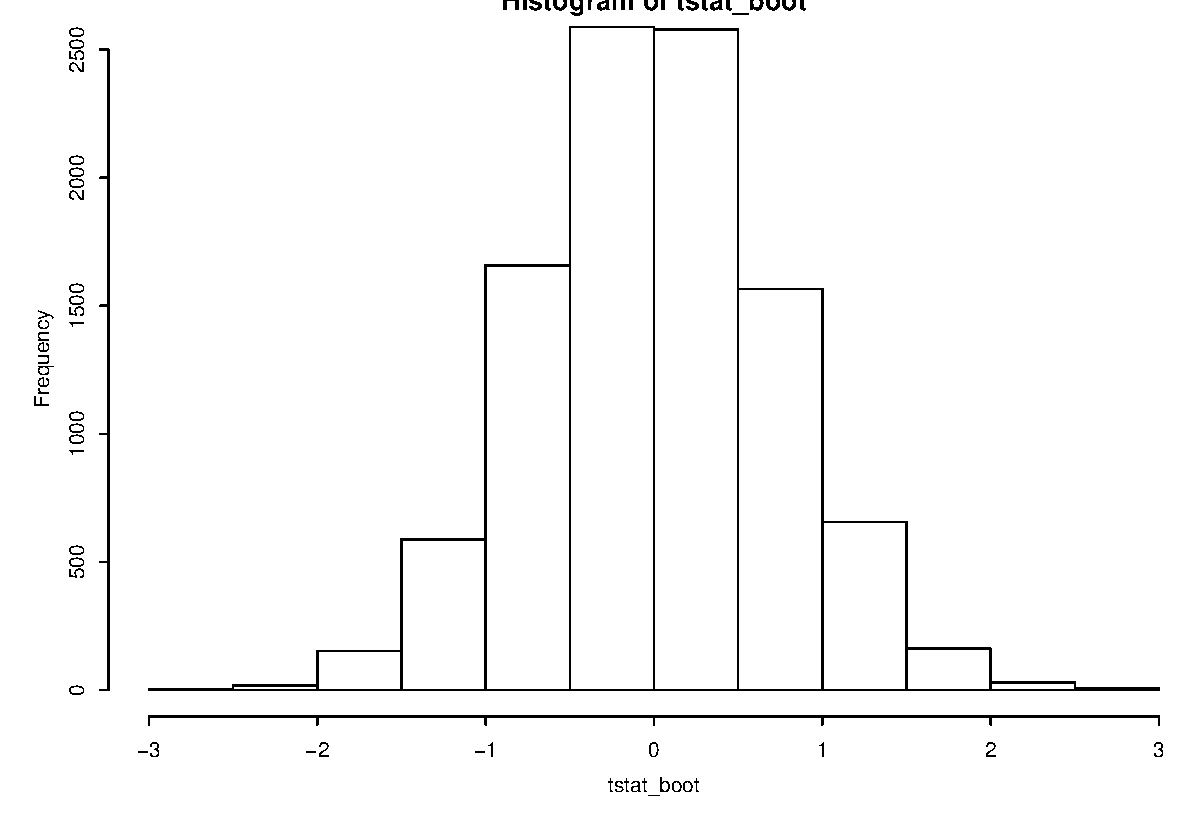
\includegraphics[width=0.99\linewidth]{figure/graphics-unnamed-chunk-12-1} 

}



\end{knitrout}

\end{frame}
%%%%%%%%%%%%%%%%%%%%%%%%%%%%%%%%%%%%%%%%%%%%%

%%%%%%%%%%%%%%%%%%%%%%%%%%%%%%%%%%%%%%%%%%%%%
\begin{frame}[fragile]
%%%%%%%%%%%%%%%%%%%%%%%%%%%%%%%%%%%%%%%%%%%%%
\frametitle{qqplot with t(51.9)}

\begin{knitrout}\small
\definecolor{shadecolor}{rgb}{1, 1, 1}\color{fgcolor}\begin{kframe}
\begin{alltt}
\hlkwd{library}\hlstd{(gap)}
\hlkwd{qqfun}\hlstd{(tstat_boot,} \hlstr{"t"}\hlstd{,} \hlkwc{df}\hlstd{=}\hlnum{51.9}\hlstd{)}
\end{alltt}
\end{kframe}

{\centering 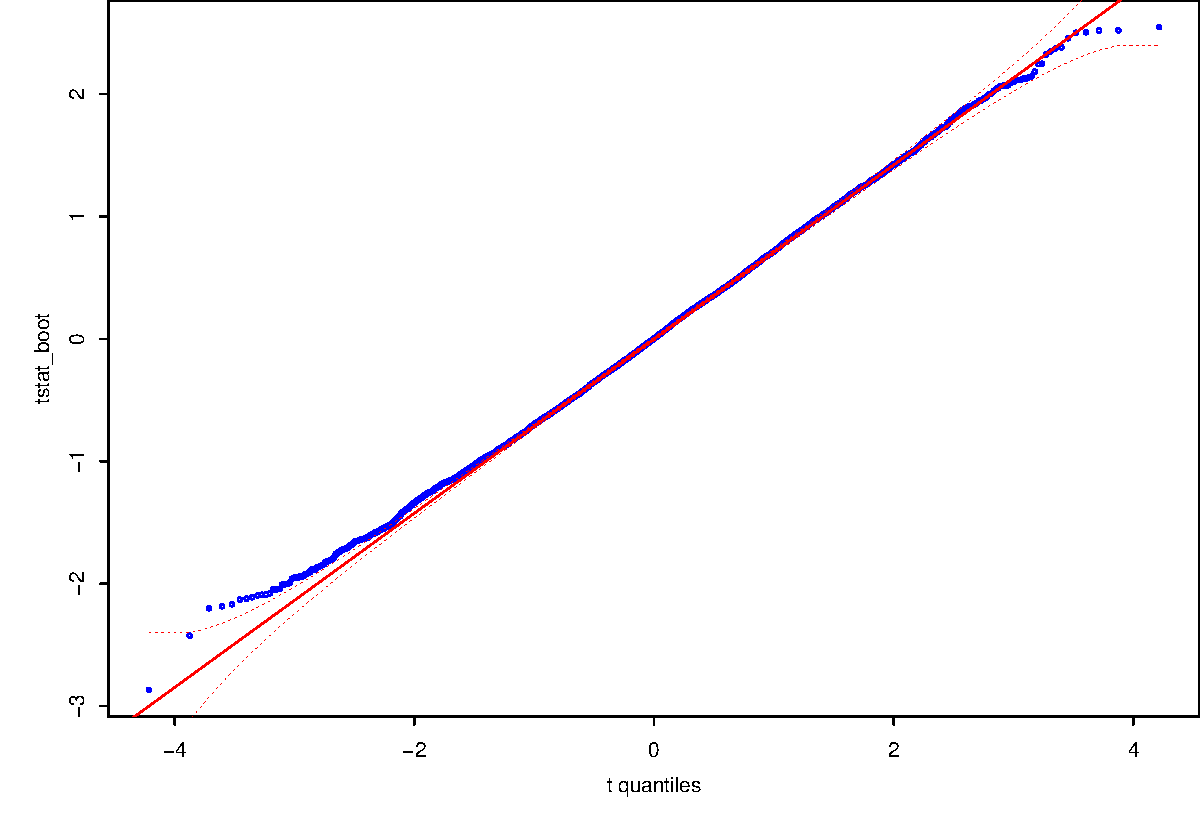
\includegraphics[width=0.99\linewidth]{figure/graphics-unnamed-chunk-13-1} 

}



\end{knitrout}

\end{frame}
%%%%%%%%%%%%%%%%%%%%%%%%%%%%%%%%%%%%%%%%%%%%%

%%%%%%%%%%%%%%%%%%%%%%%%%%%%%%%%%%%%%%%%%%%%%
\begin{frame}[fragile]
%%%%%%%%%%%%%%%%%%%%%%%%%%%%%%%%%%%%%%%%%%%%%

How to know when to assume $\sigma_1 = \sigma_2 = \sigma$. \pause \newline

The rule is  - is the ratio of sample variances less than $2$. \pause \newline

if $\frac{largest{s^2_X, s^2_Y}}{smallest{s^2_X, s^2_Y}} < 2$, then assume $\sigma_X = \sigma_Y = \sigma$. \pause \newline

When we hold this assumption to be true, we do the t-test for same $\sigma$, else the Welch method t-test.

\end{frame}
%%%%%%%%%%%%%%%%%%%%%%%%%%%%%%%%%%%%%%%%%%%%%


\end{document}
